%%%%%%%%%%%%%%%%%%%%%%%%%%%%%%%%%%%%%%%%%%
\chapter{Introduction} \label{sec:introduction}
%%%%%%%%%%%%%%%%%%%%%%%%%%%%%%%%%%%%%%%%%%
The controlled, sustained thermonuclear fusion of light elements can serve as the ultimate energy source on Earth; it is inexhaustible (on our planetary scales), produces none of the greenhouse gases that are altering our climate, and avoids many of the dangers of nuclear fission. Overcoming the engineering obstacles to tame the fusion reaction is the greatest technological challenge of our generation. %A recently-published book by Dr. Francis Chen provides an excellent coverage of the basics of fusion energy, the reactions, our present understanding of the fusion plasma, and the role fusion energy can play in the global energy market.\cite{Chen2011} 

In this dissertation, I will begin by presenting an extremely brief summary on the background of general fusion technology -- necessary for establishing a common language that will be used in the rest of the document. I'll then give slightly more background on some fusion nuclear technology that are immediately relevant to the research I have performed, specifically the breeder blanket of a fusion reactor.

\section{The Basics of Nuclear Fusion and Tritium Breeding}\label{sec:fusion-basics}

The fusion reaction chosen for the first demonstrable fusion power plants involves the two hydrogen isotopes of deuterium and tritium. The deuterium-tritium (DT) reaction has a high reaction probability at the lowest ion temperature and a high energy yield. Alternative fusion reactions of two deuterium atoms or a deuterium atom with helium-3 are advantageous in other regards, such as no radioactive byproducts or fuel availability, but their relatively-higher ion temperature preclude them from current feasibility.\cite{abdou} The DT reaction proceeds as
\begin{align}
	\mathrm{D} + \mathrm{T}&\xrightarrow{}\ ^4\mathrm{He}+\mathrm{n}+17.58\ \text{MeV} \label{eq:dt-reaction}
\end{align}

Of the two isotopes fused, deuterium ($D$, or $^2$H) is a stable isotope and is naturally occurring in an average abundance of 0.015 mole percent in water on Earth. To demonstrate just how plentiful deuterium is as a fuel source, there is approximately 100 million billion kilograms of deuterium in the Earth's oceans. If all energy on Earth were produced from DT fusion power plants, there would be enough deuterium to outlast the lifetime of our sun. It is safe to say we will not exhaust our deuterium sources on Earth.

Tritium ($T$, or $^3$H), however, is radioactive with a half-life of only about 12 years; any naturally occurring tritium decays at such a rapid pace it will never accumulate to an appreciable amount on Earth. If tritium is to be used as a fuel in a fusion power plant, it must be generated artificially. In-situ generation of tritium in a fusion reactor is possible with the assistance of lithium. Natural lithium will interact with neutrons as
\begin{subequations}\label{eq:lithium-t}
\begin{align}
	\mathrm{n} + \ ^7\mathrm{Li} &\xrightarrow \ \mathrm{n}+\alpha + \mathrm{T} -2.47\ \text{MeV}\label{eq:li7-t}\\
	\mathrm{n} + \ ^6\mathrm{Li} &\xrightarrow \  \alpha + \mathrm{T} +4.78\ \text{MeV} \label{eq:li6-t}
\end{align}
\end{subequations}
using the common short-hand of $\alpha$ in place of the helium nucleus. The cross-sections of the lithium reactions are given in Fig.~\ref{fig:li-xsects}. Of note in Fig.~\ref{fig:li-xsects} is the exothermic lithium-6 reaction (a neutron of any energy will incite the transmutation) and the threshold energy required of the incident neutron to incite the endothermic lithium-7 reaction. The exothermic reaction, in addition to producing tritium, is also the source of energy that will ultimately generate the electricity of the fusion power plant.

\begin{figure}[ht]
	\centering
	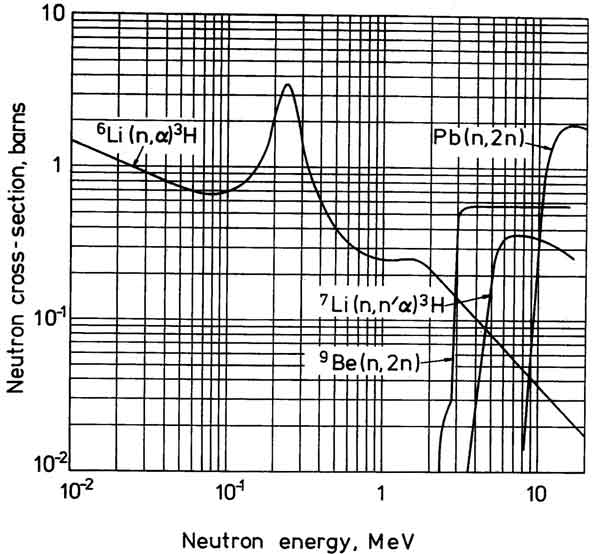
\includegraphics[width=\singleimagewidth]{chapters/figures/breeding_xsecs} 
	\caption{Cross-sections of various blanket materials. Note the threshold for the $^7$Li and neutron multiplying reactions.}
	\label{fig:li-xsects}
\end{figure}

Fortunately, lithium, like deuterium, is quite abundant on Earth. There is enough lithium accessible in the Earth's crust to generate tritium for 30 million years worth of DT reactions.\cite{Chen2011}. Thus lithium is an excellent candidate for generating the tritium necessary to self-sustain the fusion reaction in a power plant. Fusion reactor designs include so-called tritium breeding blankets which surround the plasma volume with lithium, however the form of lithium as it exists in the breeding blanket is a source of continued research.



At present there are two main concepts for tritium breeder designs: those containing liquid or solid lithium. Many of the functional requirements are similar between the two designs but their implementations are quite different. While much research has been -- and continues to be -- performed on the liquid breeder design (for examples, see Refs.~\cite{Hartmann1937,Hunt2006,Shercliff1953,Sommeria1982,Xv1937,Alfve1942}), the work of this dissertation focuses solely on the reference solid breeder design. In the next section, while introducing the breeding blanket, I will refer to the blanket almost exclusively as simply ``solid breeder'' though it should be understood that many of the generic features and requirements of the solid breeder are shared with its sister design, the liquid breeder.

\subsection{Breeding Blanket for Fusion Reactors}


\begin{figure}[ht]
	\centering
	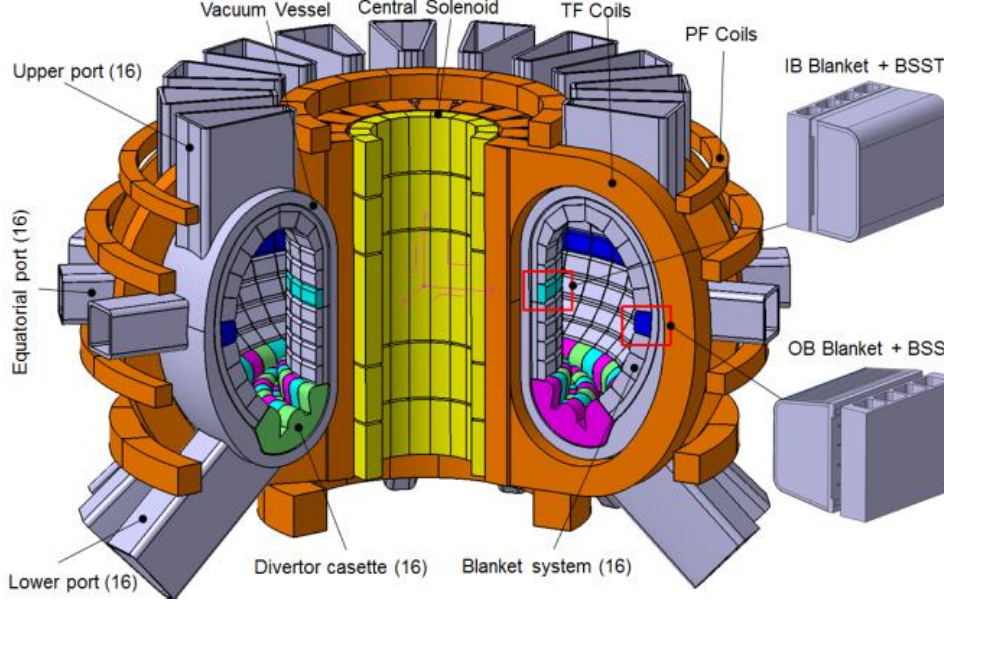
\includegraphics[width=1\textwidth]{chapters/figures/demo} 
	\caption{An example design of a DEMO reactor with solid breeder blankets shown as inboard (IB) and outboard (OB) blanket components.}
	\label{fig:demo}
\end{figure}

\begin{figure}[ht]
	\centering
	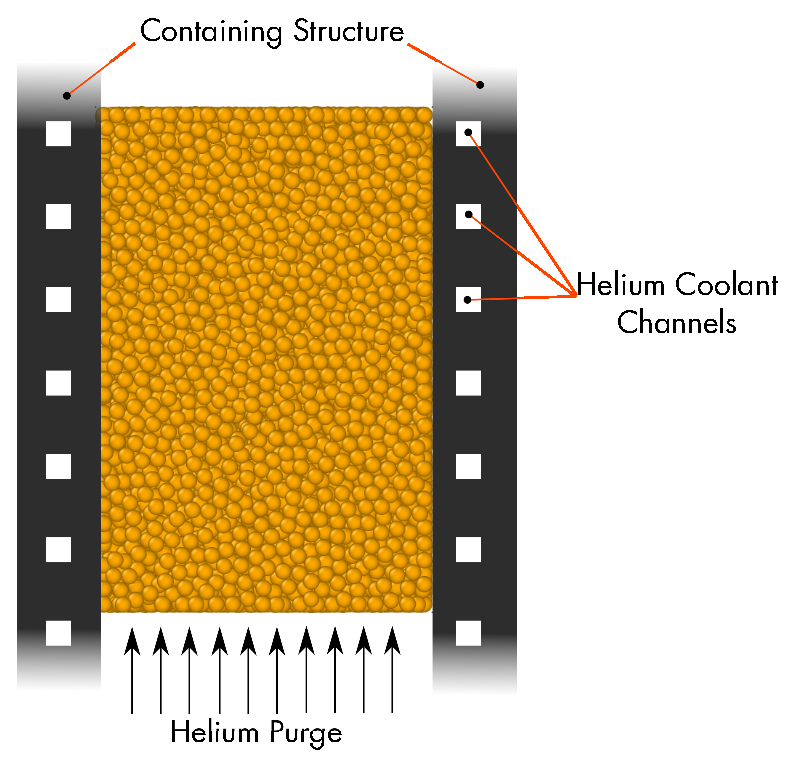
\includegraphics[width=\singleimagewidth]{chapters/figures/solid_breeder_sketch} 
	\caption{Sketch of a typical unit of a pebble bed tritium breeding zone. The pebble bed is cooled with contact to the containing structure.}
	\label{fig:solid-breeder-sketch}
\end{figure}

The breeder blanket is a critical piece of engineering technology upon which the success of a fusion power plant largely rests. The successful operation of a breeder will see the device capture the neutrons ejected from the fusion reaction to generate fuel for future reactions, act as shield to other sensitive equipment and personnel, and convert energy into extractable heat for electricity production. Figure~\ref{fig:demo} shows an example sketch of a demonstration (DEMO) fusion reactor and the relative location of the breeder blanket modules as they face the plasma in the torus of the tokamak. 

From the inception of the solid breeder concept in 1975 by Abdou\etal\cite{Abdou1975c}, designs have evolved significantly in response to requirements of operation in the harsh fusion environment. Currently, the reference solid breeder design incorporates packed beds of ceramic pebbles (spherical particles) that are filled into containment structures of volumes optimized for thermophysical and tritium responses. 

The pebble bed form has ultimately become the design of choice based on many of its attractive features. Many requirements of a solid breeder `material' (the volume of a pebble bed is often considered as a single fictitious material) are satisfied by the ceramic pebble bed. The small pebbles provide a sufficient surface-area to volume ratio; have good and customizable (via polydispersity) open-porosity to allow the helium purge gas to wind through and pick up any generated tritium from the solid; and the small size of the pebbles prevent any large thermal gradients from emerging across any single solid material object -- thus increasing the mechanical survivability of the ceramic. 

The representative pebble bed, as sketched in Fig.~\ref{fig:solid-breeder-sketch}, is shown to be contained by a low-activation steel which serves as both mechanical and thermal boundaries for the ensemble. The breeding blanket will experience high volumetric heating (resulting from secondary $\gamma$ rays and the kinetic energy of neutrons that are carrying away approximately 80\% of the fusion reaction) and temperatures will be allowed to increase to approximately 900~\celsius. The heat is conducted via inter-particle contacts between pebbles, contact with the structural material, and convection to the purge gas then transported to the structural material. A high pressure (approximately 8 MPa) helium coolant is then run through the structure. The coolant will heat to approximately 500~\celsius~before exiting the blanket, maintaining the steel below structural temperature limits. The heat carried away by the coolant ultimately works its way into an electricity-producing cycle. 

As the neutrons bombard the lithiated ceramic, tritium is produced internal to the pebbles. Tritium that transmutes from the lithium inside the pebble will diffuse slowly through the bulk until reaching a grain boundary. Tritium moves relatively quickly along the grain boundary until reaching a surface of open porosity where it may desorb into the passing purge gas.\cite{Federici1990} The low-pressure, low-speed purge gas is pumped through the pebble bed to extract the tritium generated and transport it out of the blanket for processing. 

The dual role of the breeding blanket to generate heat and tritium forces a specific operational temperature window for the ceramic pebble beds. The low end of the temperature window is governed by a minimum temperature for acceptable release rates of tritium from the ceramic to the purge gas; the value is generally set around 300~\celsius. Based on the current understanding of tritium release from the pebble, as grains grow during sintering of the ceramics the tritium release rate is expected to decrease beyond acceptable limits. Thus the upper limit of the temperature window is chosen to avoid sintering of the lithiated ceramic, giving the approximately 900~\celsius~limit mentioned previously. 

\begin{figure}
        \centering
        \begin{subfigure}[b]{\doubleimagewidth}
                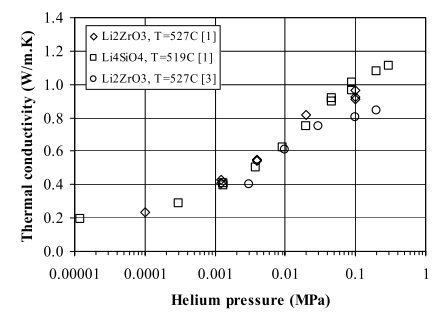
\includegraphics[width=\textwidth]{chapters/figures/keff-pressure}
                \caption{Effective conductivity of ceramic pebble beds is dependent on the pressure of the interstitial gas, a minimum of about $\keff = 1$~W/m-K in vacuum.}
                \label{fig:keff-pressure}
        \end{subfigure}%
        
          %add desired spacing between images, e. g. ~, \quad, \qquad, \hfill etc.
          %(or a blank line to force the subfigure onto a new line)
        \begin{subfigure}[b]{\doubleimagewidth 	}
                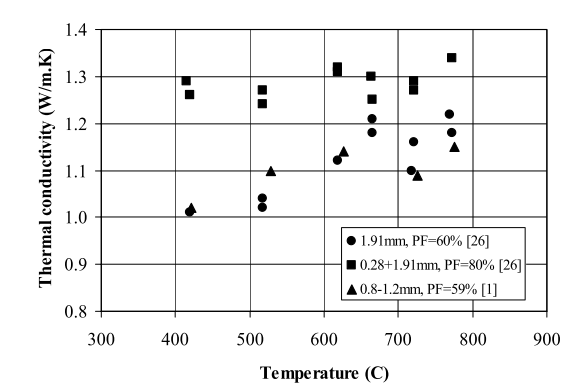
\includegraphics[width=\textwidth]{chapters/figures/lit-keff-exp}
                \caption{The effective conductivity of pebble beds is weakly dependent on external mechanical pressure and is always approximately $\keff = 1$~W/m-K in helium.}
                \label{fig:keff-lit}
        \end{subfigure}
        \caption{Effective conductivity of lithium ceramics. Results from Ref.~\cite{Abou-Sena2005}}\label{fig:keff}
\end{figure}

Many experiments have been run to measure the effective thermal conductivity of a volume of ceramic pebbles. In Figs.~\ref{fig:keff}, the effective conductivity is seen to be strongly affected by the interstitial gas but weakly affected by the mechanical loads on the bed. The main conclusions to bear in mind from Fig.~\ref{fig:keff} are that: 1) the interstitial gas is an important transporter of heat in the bed and 2) the effective thermal conductivity of the pebble bed is low and will limit the size of the ceramic pebble bed volume to satisfy the temperature window mentioned above.

% The size of breeder region is limited by the operational temperature window that must be held in spite of the the poor effective conductivity of packed beds of ceramic pebbles. The conductivity is experimentally shown to be a weak function of external pressure but can generally no greater than about \si{1 W/{mK}} -- for well-packed beds. Because the effective conductivity and packed bed-wall interface conductance is predominately a contact conduction, disruptions to the packing structure will have considerable impact on the heat transfer of the packed bed.

As nuclear energy is deposited into the poorly-conductive ceramic breeder material and the temperature climbs well above the containing structure, the pebbles will each individually begin to grow from thermal expansion. The containing structure will confine the thermal expansion of the lithium ceramic and therefore lead to large mechanical stresses at the points of contact of the individual pebbles in the packed bed. As a ceramic material, the pebbles are prone to brittle failure when the contact forces grow large. But the ceramic pebble beds must be able to survive the high temperature, high stress, and irradiated environment while providing a reliable amount of tritium to the fuel processing equipment.




 % the fusion reaction deposits   The nuclear heat generated in the pebble bed solid breeder will heat the ceramic pebbles to maximum temperatures of approximately 900~\celsius. The heat of the pebbles is transported through them via conduction through inter-particle contacts, conduction through the purge gas into neighboring particles, and ultimately through contact with the containing structure. The box structure surrounding the solid breeder will have high pressure (\si{8~MPa} in many current designs) 


\section{Motivation}\label{sec:motivation}

\begin{figure}[ht]
	\centering
	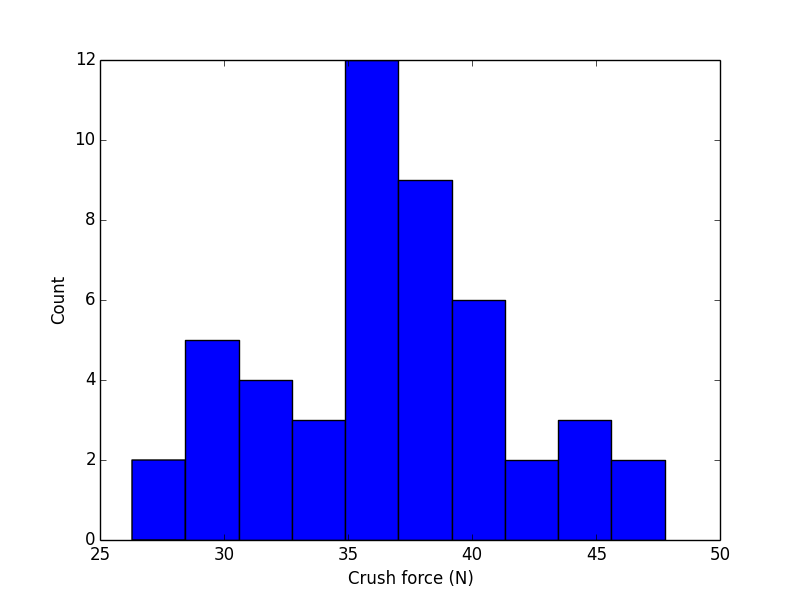
\includegraphics[width=\singleimagewidth]{chapters/figures/fmax} 
	\caption{Crush load distribution for a batch of $d_p = 1$~mm \lit pebbles.}
	\label{fig:fmax}
\end{figure}


Experiments on individual particles betray the brittle nature of ceramic pebbles and their propensity to break at relatively low individual contact forces. An example histogram of the crush loads of a batch of 1~mm \lit pebbles, as measured in our lab, is shown in Fig.~\ref{fig:fmax}. For these particular pebbles, the average crush load was less than 40 N. For some \lis pebbles, the average crush load is measured as low as 10 N. The relatively low force required to crush, coupled with the strong macroscopic loads predicted by the FEM models, brings into question the survivability of the pebbles and packing of the solid breeder.

If individual pebbles in the packed bed ensemble begin to crush, it may result in a number of negative effects on the bed. First, from Fig.~\ref{fig:keff-pressure}, we can see that a significant amount of heat (roughly 20\%) is transported through the bed purely via contact conductance between pebbles. In response to damaged pebbles, the bed will resettle from the imbalance of inter-particle and gravity forces. Any disruption in the contact network will have an impact on the heat paths internally and at the bed-wall interface. A bed with damaged pebbles could have significantly different effective thermophysical properties than those predicted for the original bed, potentially increasing the overall temperature of the bed past the acceptable temperature windows described in the previous section. Furthermore, the neutron absorption/shielding function of the solid breeder is dependent on an assumption of homogeneous distributions of pebbles in the breeding unit volume. Broken pebble fragments will settle, in time, in the direction of gravity and accumulate at the floor of the pebble bed, concurrently the entire bed may be resettling and a physical gap at the top of the pebble bed can form. This would result in undesirable quantities of neutrons streaming past the solid breeder volume. 

As the thermophysical properties evolve, global or local bed temperatures change and ultimately the tritium release characteristics of the bed deviate from any prediction one may have had from the initial packing of the ceramic pebble bed. The ceramic solid breeder must continue operating despite the harsh effects of existing in the fusion reactor. And it must continue operating without being replaced or actively maintained. Its important that the solid breeder not simply survive the thermal and mechanical demands of the reactor environment but continue to release predictable and acceptable amounts of tritium. 

In light of the short discussion above, it is apparent that a thorough study of pebble damage, including the loads on the pebble bed that will lead to broken pebbles as well as the pebble bed's thermophysical responses to broken pebbles, is critically needed for solid breeder design. Unfortunately, pebble bed experiments are inadequate for this need. The majority of measurements are only available for macroscopic properties (\textit{e.g.} uniaxial compression tests for stress-strain responses) or give only maximum measurements of individual pebble responses (\text{e.g.} pressure sensitive layers giving pebble pressures on a wall). The inability of physical experiments to reliably look into the transient inner structure of the pebble bed has driven past solid breeder researchers to employ pebble-scale models. Increasingly reliable and accurate models are crucial in the design of operational solid breeder blanket technologies. In this dissertation, I attempt to advance the field of solid breeder pebble-scale modeling with the introduction of new techniques and tools to incorporate the many facets of pebble damage in a solid breeder.

Briefly, I must consider why one would employ pebble-scale models versus those that are bed-scale. Afterall, the volume of a pebble in a tritium breeder is on the scale of 10$^{-9}$~m$^3$ while the typical container volume can be on the order of 10$^{-2}$~m$^3$\cite{Cho2008}.  Thus a single breeder volume will house upwards of $N = 10^7$ pebbles. Statistically then, it is reasonable to assume that continuum theory is applicable to the ensemble of pebbles. This assumption is the basis of development of finite element method (FEM) models for the breeder pebble beds. Constitutive equations are developed from experimental measurements of the macroscopic behavior of pebble beds which are fed into FEM models. The continuum assumption allows modeling the thermomechanical interaction of the entire pebble bed with the containing structure and coolant. The FEM models have been able to predict thermo-mechanical behavior with reasonable accuracy of some lab-scale experimental mock-ups of breeding units (A more thorough summary of the state of solid breeder modeling is given in \cref{sec:modeling-state}).\cite{DiMaio20081287,Zaccari20081282,Gan:2009vn} A notable result indicated by all the different FEM models is the indication that strong mechanical loads will arise throughout the pebble bed -- which will lead to many histrionic effects. But it is these very histrionic effects that FEM is, at present, incapable of modeling: pebble damage, resettling, and gap formation. The focus of this dissertation is on the histrionic effect of individual damaged pebbles and the morphological changes they induce in the pebble bed writ large. Thus I am compelled to consider the models at the scale of the individual pebbles.

\section{Scope of the Work}\label{sec:intro-scope-of-work}

In our group we identify the need to predict pebble damage in an ensemble, understand of the evolution of pebble bed morphology due to pebble damage, and analyze the impact of morphological changes on thermophysical and thermomechanical properties. To satisfy these needs, the work of this dissertation is to develop tools for modeling pebble interactions, predict pebble crushing based on the interactions, and monitor the macroscopic changes to temperatures in the bed in response to damaged pebbles. On the path of pebble-scale modeling development, I will:
\begin{enumerate}
	\item validate the Hertzian assumption for ceramic pebble interactions with single experiments on crushing pebbles,
	\item derive a criteria for pebble crushing in our numeric ensemble based on single pebble experiments,
	\item assess the impact of fragment size on packing resettling and other morphological features,
	\item calculate the evolving force network and its influence on the heat transport in the pebble bed.
\end{enumerate}

After implementing a sophisticated pebble-scale modeling tool, I will show the limitations of the micro-mechanical model when it comes to simulating the heat transfer of a ceramic pebble bed with a creeping helium purge gas. Thus I also implement some efficient bed-scale models of thermo-fluid flow coupled to/integrated with particle-scale mechanics. The steps toward achieving these models includes:
\begin{enumerate}
	\item adapting and employing two numerical schemes to study packed bed energy transfer with interstitial gas,
	\item analyze the reduction in $\keff$ due to broken pebbles,
	\item study the lumped-capacitance assumption (innate to the particle-scale modeling approach) in a packed bed with high Biot number with nuclear heating.
	\item address the overall impact of the helium purge gas on the thermal transport in a bed with evolving morphology,
\end{enumerate}

Finally, when the particle-scale model predicting and simulating pebble damage is coupled to thermo-fluid models of the helium purge through packed beds, I will use the numerical tools to judge the consequences of pebble damage on two ITER-relevant configurations of breeder volumes, applicable as guidance to solid breeder designers.



% The objective of this dissertation is to develop numerical models of ceramic pebble beds, based on first principles and experimental observations, to simulate the hysteritic evolution of pebble bed morphology and predict the subsequent changes to heat transport characteristics after thermally-induced damage to pebbles. The numerical tools are constructed in the following progression: 1. Transient DEM code of inter-particle interactions is employed to simulate packed bed restructuring in the wake of crushed pebbles in the ensemble -- and the effective thermal conductivity following the restructuring, 2. Transient, volume-averaged equations of Navier-Stokes and energy of the helium purge gas are coupled to the DEM model of pebbles to simulate conjugate heat transfer and the interstitial fluid influence on thermophysical properties after crushing events, 3) Complete simulations of the tortuous path of helium purge gas with lattice-Boltzmann models (based on the packing structure determined in DEM simulations) to expose flattened temperature profiles due to laminar mixing in the pebble bed. 

In summary, understanding the evolution of pebble bed morphology and its impact on thermophysical properties is critical for solid breeder designers. The understanding allows for temperature control of breeder pebble beds over the operational lifetime of the blanket which is crucial to the function of the solid breeder for tritium and energy generation. The tools I develop in the course of this dissertation are a necessary step toward realization of this understanding. 

One last note: there are other long-term effects expected in the materials experiencing prolonged exposure to cycling irradiation, heat, and stress that have not been discussed here. These loads can lead to thermal ratcheting, irradiation swelling, sintering, or thermally-induced creep which also lead to evolutions in thermophysical properties -- even in the absence of cracked pebbles. These phenomena need to be addressed in time but are, however, beyond the scope of this dissertation. 
% we aim to provide designers of packed beds with tools to understand how packing states may evolve from time-dependent phenomena (e.g. sintering, creep, pebble cracking, etc.). These phenomena may, for instance: decrease the effective thermal conductivity which will raise bed temperatures beyond initial predictions, produce isolated pebbles which will sinter and potentially decrease tritium release rates, or even form gaps between pebble beds and containing structures leading to divergence from properties of the initial packing of the bed.

% The objective of this work fits into the broader mission of our research group in the UCLA Fusion Science and Technology Center to develop and apply complete numerical models of ceramic pebble bed solid breeder modules. Any complete numerical model for a pebble bed would require the interaction of many sub-models or sub-functions operating at disparate scales. To demonstrate, a possible top-level algorithm could proceed in the following way: To begin, one must have knowledge of the interaction of the pebble bed with the containing structure as they exist in a fusion environment. The interactions are generally analyzed via the finite element method to find internal stresses and temperature fields of the entirety of the pebble bed and surrounding container. After the internal fields are mapped into the bed, one would use the discrete element method (DEM) to interpret the macroscopic stress fields into the inter-particle forces. With the inter-particle forces and total absorbed thermal energy calculated, a prediction of the initiation and evolution of morphological changes (i.e. crushed pebbles, sintering, creep, etc.) to each computational volume. Following this, DEM would calculate new effective properties as a result of the morphological changes to the pebble bed region. Finally, the updated bed properties would feed back into the FEM formulation to update calculations in the macroscopic stress fields. While a suite of integrated numerical tools that follows this example algorithm is the ultimate goal of our group, the work of this dissertation is focused entirely on the development of pebble-scale simulations that are predominately in the realm of the discrete element method.

% In the following subs-sections, we briefly outline the studies fitting into the scope of this dissertation. 

% \subsection*{Discrete Element Method Study on the Evolution of thermo-mechanics of a Pebble Bed Experiencing Pebble Damage}
% In the first study of \cref{sec:dem-studies}, we analyze the effective thermal conductivity of a pebble bed assuming different fractions of pebbles in the ensemble are completely crushed. The focus of this study is to 1) determine the extent of change, in aggregate, to ensemble properties due to individual pebble crushing, 2) relate the changes in effective conductivity to quantifiable pebble-scale properties (e.g. contact force, coordination number, etc.), 3) use the results to create guidelines for designers to anticipate acceptable limits of pebble loss from a thermal management point of view. For the DEM tools used in this study, the only mode of heat transfer considered is conduction between the solid particles. 


% \subsection*{Coupling DEM Models of Ceramic Breeder Pebble Beds to Thermofluid Models of Helium Purge Gas Using Volume-averaged CFD}
% In a fusion breeder, the helium purge gas winding through the interstitial gaps of the pebbles has a substantial contribution to overall heat transfer.\cite{Reimann:2002mi,Abou-Sena2005} The model of \cref{sec:dem-studies} is improved to include the flowing interstitial gas. In \cref{sec:cfd-dem-studies}, we continue to employ our DEM tools to provide particle-scale information such as contact force, but couple the pebbles to a volume-averaged computational fluid dynamics (CFD) code for the conjugate heat transfer simulation. The coupled CFD-DEM model is used to again simulate the heat transfer in packed beds of ceramic spheres that experience pebble crushing -- but now with a focus on highlighting the impact of a flowing interstitial helium purge gas when pebbles are crushed.


% \subsection*{Lattice-Boltzmann Method Integrating DEM Packing Structures to Study Laminar Mixing}
% The models to account for helium purge gas employed in the studies of \cref{sec:cfd-dem-studies,sec:applied-studies} assume effective drag or heat transfer coefficients for pebbles in a computational volume and then include the pebble influence through effective source/sink terms in the momentum and energy equations. The volume-averaged approach allows for simpler meshing of the fluid volume while still retaining much of the physical realism of the system. Complete models of the conjugate heat transfer of both the fluid moving through the tortuous interstitial gaps pebble beds pressing each other with small contact areas are intractable with current computational hardware and finite-element modeling techniques. To overcome deficiencies in computational power, in \cref{sec:modeling-lbm}, we apply a relatively new technique wherein a lattice-Boltzmann algorithm solves for complete flow fields and conjugate heat transfer of helium winding through a packed bed. The lattice-Boltzmann method (LBM) is a non-traditional fluid simulation technique that allows us to resolve pebble/pore-scale momentum and energy transfer. The LBM approach is applied to the same pebble beds analyzed in \cref{sec:cfd-dem-studies} to provide comparison between the two modeling techniques. Furthermore the LBM model, accounting for the complex helium purge gas pathways, provides more insight to the influence of helium on the heat transfer in the heat transfer of packed beds.





% \subsection*{Modeling Tools to Study Coolant Designs of ITER Solid Breeder Module Volumes}
% In the study of \cref{sec:applied-studies}, we apply our coupled helium-pebble computational tools to the analysis of ITER-relevant solid breeder geometries. In this study we consider the combined effects of pebble crushing, packing restructuring due to both gravity and the unbalanced force network in the pebble bed, and convection from helium purge gas on temperature profiles in solid breeders for different breeding configurations. Heat transfer out of the pebble bed relies on maintaining good pebble-pebble and pebble-wall contact. However, physical contact is interrupted to different degrees when a pebble bed responds to various amounts of individual crushed pebbles. Furthermore, the restructuring of the pebble bed after a pebble crushing event is, in part, dependent on gravity forces acting upon each pebble in the ensemble. We investigate two representative pebble bed configurations where heat is removed from the bed via inter-particle conduction, convection of purge gas, and contact between the pebble bed and its container. In the first, the coolant containing structural walls (heat transfer walls) are oriented parallel to the gravity vector. In the second configuration, the heat transfer walls are perpendicular to the direction of gravity. To simulate a crushed pebble, we replace the pebble with many smaller, non-cohesive elements while maintaining mass-conservation between the original solid pebble and crushed fragments. The fragments are then free to resettle into interstitial gaps and the rest of the bed resettles as determined by forces from gravity, contact of neighboring particles, and even the small influence of the moving purge gas. The thermo-fluid interaction with the helium purge gas will be included with volume-averaged Navier-Stokes and energy equations. The representative solid breeder volumes will be compared with respect to their temperature peaks and profiles and how those temperatures vary as a function of the percentage of crushed pebbles in the ensemble. The results can be used to optimize solid breeder pebble bed designs through the choice of breeding zone orientation relative to the gravity vector.



% \chapter{Dissertation Outline}
% The path toward the modeling efforts outlined for the scope of this work is not a clear, straight line. To accomplish the goals set forth -- attempting to discuss them in the most clear and accurate way possible -- this dissertation is broken up into five major parts following their logical partitions. This section, Part I, provides the introduction and motivation behind the work. In Part II, (containing Chapters: \cref{sec:hertz-theory,sec:modeling-state,sec:survey-packed-beds}) we survey the state of the art in analysis of ceramic pebble beds, contact mechanics, and modeling thermal and mechanical interactions of particles in packed beds and fluids moving interstitially.  In Part III, (containing Chapters: \cref{sec:modeling-dem,sec:modeling-cfd-dem,sec:modeling-lbm}) we outline the numerical methodology and development of modeling tools we shall use in the study and analysis of pebble beds and their evolving morphology due to external loads. We compartmentalize the numerical tools into three parts, namely: the discrete element method (DEM), coupled computational fluid dynamics and the discrete element method (CFD-DEM), and a lattice-Boltzmann method (LBM) we integrate with DEM. The development of the tools is assisted with theoretically- and experimentally-based studies on individual pebbles in an ensemble. The newly developed enhancements to the numerical tools are studied before their inclusion in the toolkits. We work through the results of the promised studies in Part IV (\cref{sec:cfd-dem-studies,sec:dem-studies,sec:lbm-studies,sec:applied-studies}). Finally, in Part V, we discuss the next steps to be taken that we identify as critical next steps -- but beyond the scope of this dissertation -- for the modeling tools. In addition, other research avenues that have been opened by the tools introduced and their potential impact are discussed here.